\section{Deep Learning on Graphs}
\label{s_Background}

The foundation of this research lies at the intersection of graph theory, machine learning, and temporal data analysis. 
%This chapter provides a comprehensive overview of the key concepts and methodologies that underpin the thesis, and introduces the notation used throughout the thesis. 
This chapter acts as a guide, leading the reader through the key concepts and methodologies that underpin this thesis. A core preliminary for explaining deep graph models on dynamic graphs lies in dynamic graphs themselves. Thus, chapter \ref{s_Background_Graphs} establishes the definitions and fundamental differences between static and dynamic graphs (Section \ref{s_Background_Graphs}). After that, geometric deep learning is outlined (Section \ref{s_Background_GeometricDeepLearning}) as the basis for deep graph models, followed by an in-depth introduction to \glspl{gnn} (Section \ref{s_Background_GNNs}). Building upon this foundation, the final sub-chapter (Section \ref{s_Background_TGNNs}) covers the extension of \glspl{gnn} into the temporal domain. It introduces \gls{gnn} models designed for different representations of dynamic graphs. While Section \ref{s_Background_Graphs} introduces the notation and vocabulary used throughout this thesis, Sections \ref{s_Background_GeometricDeepLearning} - \ref{s_Background_TGNNs} introduce the concepts that underpin the explained models.

\subsection{Graphs}
\label{s_Background_Graphs}
On the most fundamental level, graphs are mathematical structures for modeling pairwise relationships between objects \cite{diestel_graph_2017}. They find application in diverse domains like social and communication networks \cite{bronstein_geometric_2017}. Graphs can be represented and denoted in a variety of ways. This thesis employs a notation based on the notation of Diestel \cite{diestel_graph_2017}, You et al. \cite{you_roland_2022}, and Souza et al. \cite{souza_provably_2022} to introduce and explore essential graph-related concepts.
% Introduction into the very basic definitions of graphs

A graph is characterized as a pair $G = (V, E)$, consisting of a set of vertices ${V= \{v_1,...,v_n\}}$, also called nodes, and a multi-set of edges $E \subseteq V \times V$ \cite{diestel_graph_2017, you_roland_2022}. Each edge $e_i \in E$ is associated with two vertices, which are called its ends \cite{diestel_graph_2017}. If a vertex $v_j \in V$ is the end to an edge $e_i \in E$, then $v_j$ is designated as incident to $e_i$ \cite{diestel_graph_2017}. An edge $e_i \in E$ connecting a node $v_j \in V$ with itself is called a loop \cite{diestel_graph_2017}. Another vertex $v_k \in V$ is adjacent, or a neighbor, to vertex $v_j$ if they are connected by an edge \cite{diestel_graph_2017}. 

Two vertices $v_0, v_n \in V$ can be linked by a walk $W(v_0, v_n)$, which is an alternating sequence of vertices and edges $W(v_0, v_n)=(v_0, e_0, v_1, ..., e_n, v_n)$ so that for all $j=1,..,n$ the nodes $v_{j-1}$ and $v_j$ are the end points of edge $e_j$ \cite{diestel_graph_2017}. The length of a walk is the number of edges in the walk \cite{diestel_graph_2017}.
% In the context of this work, we are interested in graphs that exhibit specific characteristics

Furthermore, there exist different fundamental graph types. The graph types provide a richer vocabulary for modeling complex relationships and structures. The important graph types in the scope of this thesis are listed in the following.

\begin{itemize}
    \item In a \textbf{directed graph} each edge $e_i \in E$ connecting vertices $v_j \in V$ and $v_k \in V$ has a designated stating point and end point \cite{diestel_graph_2017}. Therefore, each edge is represented as tuple $e_i = (v_j, v_k)$ with initial vertex $v_j$ and terminal vertex $v_k$. 
    
    \item In an \textbf{undirected graph}, edges have no direction, meaning that edge $e_i \in E$ connecting vertices $v_j \in V$ and $v_k \in V$ is represented as set $e = \{v_j, v_k\}$.
    
    \item A \textbf{multigraph} is a type of graph where multi-edges are permitted. This means that for any edge $e_i = (v_j,v_k) \in E$, there can exist multiple other edges $e_l = (v_j,v_k) \in E$ that share the same ends \cite{kazemi_representation_2019}.
    
    \item An \textbf{attributed} graph associates properties with vertices and/or edges to represent their characteristics \cite{kazemi_representation_2019}. Node attributes are denoted as $A^{vertex} = \{a^{vertex}_{v_i} | v_i \in V\}$, and edge attributes as $A^{edge} = \{a^{edge}_{e_i} | e_i \in E\}$. The attributes are also referred to as features.
    
    \item A graph is called \textbf{$r$-partite} if the node set $V$ can be partitioned into $r$ classes so that all edges have their ends in different classes \cite{diestel_graph_2017}. A $2$-partite graph is generally referred to as \textbf{bipartite} graph \cite{diestel_graph_2017}.
\end{itemize}

Figure \ref{f_graphs} shows examples of graphs with different characteristics. Several of these characteristics can coexist within a single graph. For example, the graph in Figure \ref{f_graphs_multi} is a directed multigraph.

\begin{figure}[ht]
    \centering
\begin{subfigure}[b]{0.45\textwidth}
    \centering
    % TikZ code for the first graph
    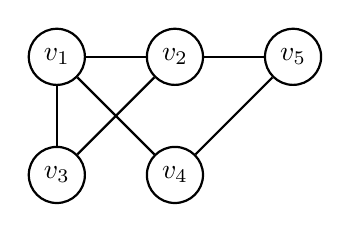
\begin{tikzpicture}[node distance={15mm}, thick, main/.style = {draw, circle}]
        \node[main] (1) {$v_1$};
        \node[main] (2) [right of=1] {$v_2$};
        \node[main] (3) [below of=1] {$v_3$};
        \node[main] (4) [below of=2] {$v_4$};
        \node[main] (5) [right of=2] {$v_5$};
        \draw (1) -- (2);
        \draw (1) -- (3);
        \draw (1) -- (4);
        \draw (2) -- (3);
        \draw (2) -- (5);
        \draw (4) -- (5);
    \end{tikzpicture}
    \caption{Undirected graph}
    \label{f_graphs_undirected}
\end{subfigure}
\begin{subfigure}[b]{0.45\textwidth}
    \centering
    % TikZ code for the second graph
    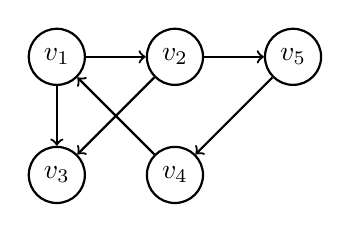
\begin{tikzpicture}[node distance={15mm}, thick, main/.style = {draw, circle}]
        \node[main] (1) {$v_1$};
        \node[main] (2) [right of=1] {$v_2$};
        \node[main] (3) [below of=1] {$v_3$};
        \node[main] (4) [below of=2] {$v_4$};
        \node[main] (5) [right of=2] {$v_5$};
        \draw[->] (1) -- (2);
        \draw[->] (1) -- (3);
        \draw[->] (4) -- (1);
        \draw[->] (2) -- (3);
        \draw[->] (2) -- (5);
        \draw[->] (5) -- (4);
    \end{tikzpicture}
    \caption{Directed graph}
    \label{f_graphs_directed}
\end{subfigure}
\par\bigskip
\begin{subfigure}[b]{0.45\textwidth}
    \centering
    % TikZ code for the first graph
    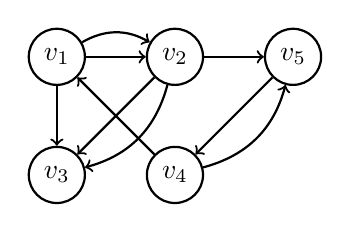
\begin{tikzpicture}[node distance={15mm}, thick, main/.style = {draw, circle}]
        \node[main] (1) {$v_1$};
        \node[main] (2) [right of=1] {$v_2$};
        \node[main] (3) [below of=1] {$v_3$};
        \node[main] (4) [below of=2] {$v_4$};
        \node[main] (5) [right of=2] {$v_5$};
        \draw[->] (1) -- (2);
        \draw[->] (1) to[bend left] (2);
        \draw[->] (1) -- (3);
        \draw[->] (4) -- (1);
        \draw[->] (2) -- (3);
        \draw[->] (2) to[bend left] (3);
        \draw[->] (2) -- (5);
        \draw[->] (5) -- (4);
        \draw[->] (4) to[bend right] (5);
    \end{tikzpicture}
    \caption{Multigraph}
    \label{f_graphs_multi}
\end{subfigure}
\begin{subfigure}[b]{0.45\textwidth}
    \centering
    % TikZ code for the second graph
    \begin{tikzpicture}[node distance={15mm}, thick, main/.style = {draw, circle}]
        \node[main] (1) {$v_1$};
        \node[main] (2) [right of=1] {$v_2$};
        \node[main] (3) [below of=1] {$v_3$};
        \node[main] (4) [below of=2] {$v_4$};
        
        \node[draw, rectangle, left=1mm of 1] {$f_{v_1}=[...]$};
        \node[draw, rectangle, right=1mm of 2] {$f_{v_2}=[...]$};
        \node[draw, rectangle, left=1mm of 3] {$f_{v_3}=[...]$};
        \node[draw, rectangle, right=1mm of 4] {$f_{v_4}=[...]$};
        
        \draw (1) -- (2);
        \draw (1) -- (3);
        \draw (4) -- (1);
        \draw (2) -- (3);
    \end{tikzpicture}
    \caption{Attributed graph}
    \label{f_graphs_attributed}
\end{subfigure}
\par\bigskip
\begin{subfigure}[b]{0.45\textwidth}
    \centering
    % TikZ code for the first graph
    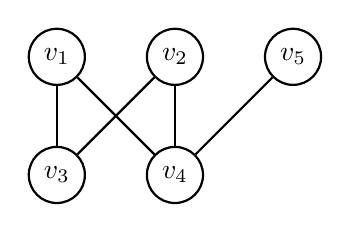
\begin{tikzpicture}[node distance={15mm}, thick, main/.style = {draw, circle}]
        \node[main] (1) {$v_1$};
        \node[main] (2) [right of=1] {$v_2$};
        \node[main] (3) [below of=1] {$v_3$};
        \node[main] (4) [below of=2] {$v_4$};
        \node[main] (5) [right of=2] {$v_5$};
        
        \draw (1) -- (3);
        \draw (1) -- (4);
        \draw (2) -- (3);
        \draw (2) -- (4);
        \draw (4) -- (5);
    \end{tikzpicture}
    \caption{Bipartite graph}
    \label{f_graphs_bipartite}
\end{subfigure}
\begin{subfigure}[b]{0.45\textwidth}
    \centering
    % TikZ code for the second graph
    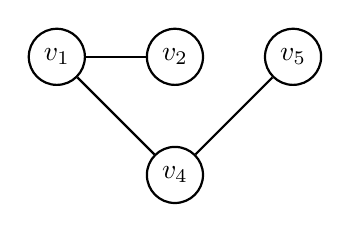
\begin{tikzpicture}[node distance={15mm}, thick, main/.style = {draw, circle}]
        \node[main] (1) {$v_1$};
        \node[main] (2) [right of=1] {$v_2$};
        \node[main] (4) [below of=2] {$v_4$};
        \node[main] (5) [right of=2] {$v_5$};
        \draw (1) -- (2);
        \draw (4) -- (1);
        \draw (5) -- (4);
    \end{tikzpicture}
    \caption{Subgraph of graph (a)}
    \label{f_graphs_subgraph}
\end{subfigure}    
    % Add more subfigures as needed
    \caption{Examples of different graphs. Graphs (a) to (e) exhibit different characteristics, and graph (f) is a subgraph of the undirected graph (a).}
    \label{f_graphs}
\end{figure}

Another critical aspect of graph theory is the concept of subgraphs. A graph $G' = (V', E')$ is called a subgraph of $G = (V,E)$ if $V' \subseteq V$ and $E' \subseteq E$ \cite{diestel_graph_2017}. For example, Figure \ref{f_graphs_subgraph} portrays a subgraph derived from the graph in Figure \ref{f_graphs_undirected}. 

%In the application of functions on graphs, an important type of a subgraph is the local neighborhood of a node. - Not really a subgraph though
In addition to the structural definitions of graphs, there are further graph-related concepts that are important in the scope of this work. A fundamental concept is the local neighborhood $N_1(v_i) = \{v_j \in V | (v_i, v_j) \in E\}$ of a node $v_i \in V$, which consists of those nodes that are adjacent to $v_i$.
%For a node $v_i \in V$, the local neighborhood $N_1(v_i) = \{v_j \in V | (v_i, v_j) \in E\}$ \cite{wu_comprehensive_2021} consists of those nodes adjacent to $v_i$. 
The local neighborhood $N_1(v_i)$ is also referred to as the $1$-hop-neighborhood of $v_i$ because it exclusively contains nodes at a distance of $1$ edge from $v_i$ \cite{bronstein_geometric_2021}. More broadly, the $k$-hop-neighborhood $N_k(v_i)$ of a node $v_i$ encompasses nodes connected to $v_i$ by walks with a length of at most $k$. 

% Wrap up by transitioning to static graphs

%As previously discussed, graphs provide a foundational framework for representing relationships between objects. Describing these connections as sets of nodes and edges allows modeling data from many different domains and with various shapes and forms \cite{bronstein_geometric_2017, kazemi_representation_2019}. Such graphs are commonly known as static graphs \cite{kazemi_representation_2019, rossi_temporal_2020, you_roland_2022} because they capture relationships that remain constant. 

The graphs presented up to this point are commonly referred to as static graphs \cite{kazemi_representation_2019, rossi_temporal_2020, you_roland_2022} because they capture relationships that remain constant. However, the real world rarely remains static; it continuously evolves, adapts, and undergoes change. To address the need for modeling these dynamic transformations, the concepts of static graphs are extended by a temporal dimension to encompass so-called dynamic graphs. Dynamic graphs introduce the element of time, allowing the capture of how relationships evolve and persist over time. In doing so, they provide a richer, more nuanced understanding of interconnected systems, closely mirroring real-world processes \cite{you_roland_2022, xu_inductive_2020, trivedi_dyrep_2019}. Examples of real-world processes that are best modeled as dynamic graphs are social networks, in which connections between individuals constantly form and end, and road networks with traffic information that continuously changes.

Two main approaches for modeling dynamic graphs have been proposed: First, modeling evolving graphs as a series of different static snapshots of a graph, so-called \acrfullpl{dtdg} \cite{he_explainer_2022, xie_explaining_2022}. Second, modeling dynamic graphs as a timed list of interaction events, so-called \acrfullpl{ctdg} \cite{rossi_temporal_2020, trivedi_dyrep_2019}. In the following sections, these approaches are explored to establish the foundation of this work.

\subsubsection{Discrete-Time Dynamic Graphs}
\label{s_Background_Graphs_DTDGs}
\glspl{dtdg} represent dynamic graphs as a series of static graph snapshots captured at different points in time \cite{rossi_temporal_2020}. These snapshots are usually taken with a constant temporal distance \cite{souza_provably_2022}. The changes between the snapshots represent the dynamic evolution of the graph. Formally, a dynamic graph in discrete-time representation is defined as $\mathcal{G} = \{G_t | t = 1,...,T\}$, where $T$ denotes the number of timestamps for which a snapshot is recorded \cite{you_roland_2022}. Each snapshot represents a static graph $G_t = (V_t, E_t)$ with a set of nodes $V_t = \{v \in V | \tau_v = t\}$ and a set of edges $E_t = \{e \in E | \tau_e = t\}$ at a specific time $t \in \{1, ..., T\}$. Each vertex $v$ and edge $e$ carries a timestamp $\tau_v$ and $\tau_e$ respectively \cite{you_roland_2022}. $V$ and $E$ represent the sets of nodes and edges aggregated across all timestamps. Furthermore, in an attributed \gls{dtdg} each snapshot is associated with node features $A_t^{vertex} = \{a_{v,t}^{vertex} | v \in V_t\}$ and edge features $A_t^{edge} = \{a_{e,t}^{edge} | e \in E_t\}$. Compared to its static counterpart, the temporal $1$-hop-neighborhood $N_1(v_i, t) = \{v_j \in V_t | (v_i, v_j) \in E_t\}$ of a node $v_i \in V$ additionally depends on the time $t$. Using the \gls{dtdg} representation, node and edge additions and deletions, as well as attribute updates to node and edge features can be modeled. Figure \ref{f_dtdg} shows an example of a \gls{dtdg}.


\begin{figure}[h]
    \centering
\begin{subfigure}[b]{0.3\textwidth}
    \centering
    % TikZ code for the first graph
    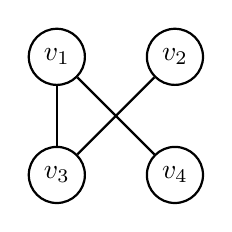
\begin{tikzpicture}[node distance={15mm}, thick, main/.style = {draw, circle}]
        \node[main] (1) {$v_1$};
        \node[main] (2) [right of=1] {$v_2$};
        \node[main] (3) [below of=1] {$v_3$};
        \node[main] (4) [below of=2] {$v_4$};
        \draw (1) -- (3);
        \draw (1) -- (4);
        \draw (2) -- (3);
    \end{tikzpicture}
    \caption{Snapshot $G_1$}
    \label{f_dtdg_1}
\end{subfigure}
\begin{subfigure}[b]{0.3\textwidth}
    \centering
    % TikZ code for the second graph
    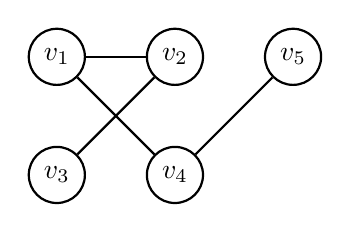
\begin{tikzpicture}[node distance={15mm}, thick, main/.style = {draw, circle}]
        \node[main] (1) {$v_1$};
        \node[main] (2) [right of=1] {$v_2$};
        \node[main] (3) [below of=1] {$v_3$};
        \node[main] (4) [below of=2] {$v_4$};
        \node[main] (5) [right of=2] {$v_5$};
        \draw (1) -- (2);
        \draw (1) -- (4);
        \draw (2) -- (3);
        \draw (4) -- (5);
    \end{tikzpicture}
    \caption{Snapshot $G_2$}
    \label{f_dtdg_2}
\end{subfigure}
\begin{subfigure}[b]{0.3\textwidth}
    \centering
    % TikZ code for the second graph
    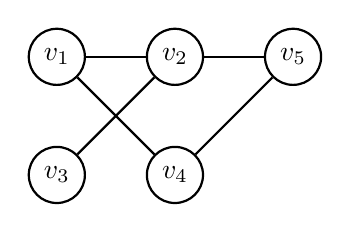
\begin{tikzpicture}[node distance={15mm}, thick, main/.style = {draw, circle}]
        \node[main] (1) {$v_1$};
        \node[main] (2) [right of=1] {$v_2$};
        \node[main] (3) [below of=1] {$v_3$};
        \node[main] (4) [below of=2] {$v_4$};
        \node[main] (5) [right of=2] {$v_5$};
        \draw (1) -- (2);
        \draw (1) -- (4);
        \draw (2) -- (3);
        \draw (2) -- (5);
        \draw (4) -- (5);
    \end{tikzpicture}
    \caption{Snapshot $G_3$}
    \label{f_dtdg_3}
\end{subfigure}
    % Add more subfigures as needed
    \caption{Example of a \gls{dtdg} $\mathcal{G}=\{G_1, G_2, G_3\}$ at different snapshots. Between $G_1$ and $G_2$ the edge $\{v_1, v_3\}$ is removed, node $v_5$ is added and edges $\{v_1, v_2\}$ and $\{v_4, v_5\}$ are added. From $G_2$ to $G_3$ another edge $\{v_2, v_5\}$ is added.}
    \label{f_dtdg}
\end{figure}

While \glspl{dtdg} offer simplicity and ease of processing through their snapshot-based representation \cite{kazemi_representation_2019}, they sacrifice detailed structural information by design, leading to a coarse depiction of temporal data \cite{trivedi_dyrep_2019, kazemi_representation_2019}. Consequently, they may struggle to capture small and irregular temporal changes \cite{trivedi_dyrep_2019, souza_provably_2022}. For example, this representation may miss the addition and prompt removal of an edge. Moreover, selecting an appropriate granularity for taking snapshots often results in suboptimal representations \cite{trivedi_dyrep_2019}. Reducing the time interval between snapshots can mitigate these limitations. Still, it introduces complexity by including the entire static graph in each snapshot, leading to parameter redundancy due to shared nodes and edges between snapshots. These shortcomings are addressed by \acrlongpl{ctdg}.

\subsubsection{Continuous-Time Dynamic Graphs}
\label{s_Background_Graphs_CTDGs}

\glspl{ctdg} offer a high temporal granularity \cite{trivedi_dyrep_2019} and are efficiently represented as sequence of timestamped events $\mathcal{G} = \{\varepsilon_{1}, \varepsilon_{2}, ...\}$ \cite{rossi_temporal_2020}. Following Rossi et al. \cite{rossi_temporal_2020}, each event $\varepsilon_{i}$ is associated with a timestamp $t_i$ with $t_1 \leq t_2 \leq ...$. 
There are node-wise events and interaction events. A node-wise event expresses the addition, removal, or attribute update of a node. Node-wise events are defined as a tuple:

\begin{equation}
    \varepsilon_{i} = (v_j, a^{vertex}_{v_j, t_i}, type_{i}, t_i)
\end{equation}

The tuple contains a timestamp $t_i$ that denotes the time at which the event happens. Further, it includes an event type ${type_{i} \in \{\mathrm{add}, \mathrm{delete}, \mathrm{update}\}}$ that describes what the event represents, e.g., either a node addition, a node deletion, or a feature update for a node. Additionally, it includes the node $v_j$ that is added, deleted, or updated, as well as its node features $a^{vertex}_{v_j, t_i}$ at that point in time. As example, the event $\varepsilon_1 = (v_1, (1,1,1), \mathrm{add}, t_1)$ describes the addition of node $v_1$ with attributes $(1,1,1)$ to the graph at time $t_1$.

An interaction event represents the addition, removal, or attribute update of an edge. Interaction events are defined as a tuple:

\begin{equation}
    \varepsilon_{i} = (e_j, a^{edge}_{e_j, t_i}, type_{i}, t_i)
\end{equation}

Similar to node-wise events, interaction events are also associated with a timestamp $t_i$ that denotes the time of the occurrence of the interaction event and an event type ${type_{i} \in \{\mathrm{add}, \mathrm{delete}, \mathrm{update}\}}$ that defines what type of an event $\varepsilon_i$ is. Interaction events include an edge $e_j$ that is part of the interaction, as well as the attributes of this edge $a^{edge}_{e_j, t_i}$. As an example, the event $\varepsilon_5 = (e_1, (1,1,1), \mathrm{add}, t_5)$ with $e_1 = (v_1, v_2)$ describes the addition of an edge $e_1$ between nodes $v_1$ and $v_2$ with attributes $(1,1,1)$ to the dynamic graph at time $t_5$.

%There are node-wise events and interaction events. A node-wise event $\varepsilon_{i} = (v_j, a^{vertex}_{v_j, t_i}, type_{i}, t_i)$ is a tuple that expresses a node addition, deletion, or feature update. The tuple contains the features of node $v_j$ at $t_i$ denoted by $a^{vertex}_{v_j, t_i}$. A node-wise event additionally is associated with an event type $type_{i} \in \{\mathrm{add}, \mathrm{delete}, \mathrm{update}\}$ that describes what the event represents. An interaction event $\varepsilon_{i} = (e_j, a^{edge}_{e_j, t_i}, type_{i}, t_i)$ signifies the addition, deletion, or feature update of an edge $e_j$. An interaction event includes the associated edge features $a^{edge}_{e_j, t_i}$ of edge $e_j$ at timestamp $t_i$ and an event type $type_{i}$. 
Depending on whether an event $\varepsilon_i$ is a node-wise event or an interaction event, it has one or two so-called involved nodes. The involved node in a node-wise event is the node that the event adds, deletes, or updates. The involved nodes in an interaction event are those two nodes that are connected by the edge that is added, deleted, or updated by the event. 

The node set $V$ and the edge set $E$ include all nodes and edges that are involved in any event in $\mathcal{G}$. A snapshot $G_{t_i} = (V_{t_i}, E_{t_i})$ of a \gls{ctdg} $\mathcal{G}$ is a representation of $\mathcal{G}$ at time $t_i$ as a static graph. $V_{t_i}$ is the node set and $E_{t_i}$ the edge set in the snapshot $G_{t_i}$. The snapshot $G_{t_i}$ at time $t_i$ is constructed from all events $\mathcal{G}(t_i) = \{\varepsilon_1, \varepsilon_2, ..., \varepsilon_i\}$ that occurred before or at timestamp $t_i$.

% For any timestamp $t_i$ a snapshot $G_{t_i}$ of $\mathcal{G}$ at that particular time is defined by all past events $\mathcal{G}(t_i) = \{\varepsilon_{j} | j = 1,...,i\}$.

As in \glspl{dtdg}, the temporal $1$-hop-neighborhood of a node $v_i \in V$ at time $t_l$ is defined as $N_1(v_i, t_l) = \{v_j \in V_{t_l} | (v_i, v_j) \in E_{t_l}\}$. The temporal-$k$-hop-neighborhood consists of those nodes $v_j \in V_{t_l}$ that are connected to $v_i$ with a walk in $E_{t_l}$ that has a length of at most $k$.

%The concept of temporal neighborhoods is extended from nodes to events. The temporal $k$-hop-neighborhood $N_k(\varepsilon_i)$ of an event $\varepsilon_{i}$ consists of those events $\varepsilon_{j} \in \mathcal{G}(t_i) \setminus \varepsilon_{i}$ for which any node involved in event $\varepsilon_{i}$ is in the temporal $k$-hop-neighborhood of any node involved in the event $\varepsilon_{j}$.

For \glspl{ctdg}, the concept of temporal neighborhoods is extended from nodes to events. The temporal $k$-hop-neighborhood $N_k(\varepsilon_i)$ of an event $\varepsilon_{i}$ consists of those past events that involve nodes that are in the temporal $k$-hop-neighborhood of the nodes involved in the event $\varepsilon_{i}$. This means an event $\varepsilon_{j} \in (\mathcal{G}(t_i) \setminus \varepsilon_{i})$ is in the temporal $k$-hop-neighborhood of $\varepsilon_{i}$ if any node involved in event $\varepsilon_{i}$ is in the temporal $k$-hop-neighborhood of any node involved in the event $\varepsilon_{j}$.

\vspace{5mm}

Table \ref{t_ctdg_events} and Figure \ref{f_ctdg} illustrate an example of a \gls{ctdg} $\mathcal{G}$, showing the events in Table \ref{t_ctdg_events} and the evolving graph in Figure \ref{f_ctdg}. Table \ref{t_ctdg_events} demonstrates that this representation provides a highly detailed yet compact representation of the dynamic graph evolution. This is a significant advantage over the representation as \gls{dtdg} \cite{trivedi_dyrep_2019}. The drawback of \glspl{ctdg} is that an evaluation of the graph's state at any given timestamp necessitates the examination of all past events and the assembly of the graph at that specific moment. In comparison, the snapshots that comprise a \gls{dtdg} already have a graph structure.

\begin{table}[ht]
    \centering
    \begin{tabular}{|l|l|}
        \hline
        Event & Description \\
        \hline
        $\varepsilon_{1} = \{v_1, a^{vertex}_{v_1, t_1}, \mathrm{add}, t_1\}$ & Add vertex $v_1$\\
        $\varepsilon_{2} = \{v_2, a^{vertex}_{v_2, t_2}, \mathrm{add}, t_2\}$ & Add vertex $v_2$\\
        $\varepsilon_{3} = \{v_3, a^{vertex}_{v_3, t_3}, \mathrm{add}, t_3\}$ & Add vertex $v_3$\\
        $\varepsilon_{4} = \{e_1 = \{v_1, v_3\}, a^{edge}_{e_1, t_4}, \mathrm{add}, t_4\}$ & Add edge $e_1$ between vertices $v_1$ and $v_3$\\
        $\varepsilon_{5} = \{e_2 = \{v_2, v_3\}, a^{edge}_{e_2, t_5}, \mathrm{add}, t_5\}$ & Add edge $e_2$ between vertices $v_3$ and $v_3$\\
        $\varepsilon_{6} = \{v_4, a^{vertex}_{v_4, t_6}, \mathrm{add}, t_6\}$ & Add vertex $v_4$\\
        $\varepsilon_{7} = \{e_1 = \{v_1, v_3\}, a^{edge}_{e_1, t_7}, \mathrm{delete}, t_7\}$ & Remove edge $e_i$ between vertices $v_1$ and $v_3$\\
        $\varepsilon_{8} = \{v_1, a^{vertex}_{v_1, t_8}, \mathrm{delete}, t_8\}$ & Remove vertex $v_1$\\
        $\vdots$ & $\vdots$ \\
    \end{tabular}
    \caption{Sequence of events comprising an example graph $\mathcal{G}.$}
    \label{t_ctdg_events}
\end{table}

\begin{figure}[ht]
    \centering
\begin{subfigure}[b]{0.3\textwidth}
    \centering
    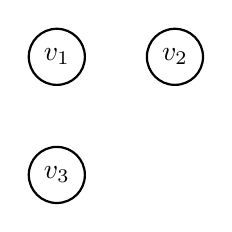
\begin{tikzpicture}[node distance={15mm}, thick, main/.style = {draw, circle}]
        \node[main] (1) {$v_1$};
        \node[main] (2) [right of=1] {$v_2$};
        \node[main] (3) [below of=1] {$v_3$};
    \end{tikzpicture}
    \caption{$G_{t_3}$}
    \label{f_ctdg_1}
\end{subfigure}
\begin{subfigure}[b]{0.3\textwidth}
    \centering
    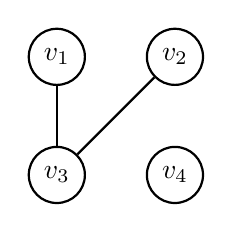
\begin{tikzpicture}[node distance={15mm}, thick, main/.style = {draw, circle}]
        \node[main] (1) {$v_1$};
        \node[main] (2) [right of=1] {$v_2$};
        \node[main] (3) [below of=1] {$v_3$};
        \node[main] (4) [below of=2] {$v_4$};
        \draw (1) -- (3);
        \draw (2) -- (3);
    \end{tikzpicture}
    \caption{$G_{t_6}$}
    \label{f_ctdg_2}
\end{subfigure}
\begin{subfigure}[b]{0.3\textwidth}
    \centering
    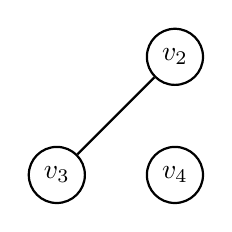
\begin{tikzpicture}[node distance={15mm}, thick, main/.style = {draw, circle}]
        \node[main] (3) {$v_3$};
        \node[main] (4) [right of=3] {$v_4$};
        \node[main] (2) [above of=4] {$v_2$};
        \draw (2) -- (3);
    \end{tikzpicture}
    \caption{$G_{t_8}$}
    \label{f_ctdg_3}
\end{subfigure}
    \caption{Different example snapshots of the graph $\mathcal{G}$ from Table \ref{t_ctdg_events} at timestamps $t_3$, $t_6$ and $t_8$.}
    \label{f_ctdg}
\end{figure}


\subsection{Geometric Deep Learning}
\label{s_Background_GeometricDeepLearning}


A major hurdle for applying deep learning methods to graphs lies in their underlying non-euclidean structure \cite{wu_comprehensive_2021}. This means that graph data cannot be mapped to an Euclidean space $\mathbb{R}^n$ (for some dimension $n$). Geometric deep learning extends deep neural networks to non-Euclidean domains, providing a framework for working with graph data \cite{bronstein_geometric_2017, bronstein_geometric_2021}. The core principle in geometric deep learning is to leverage inherent symmetries in data to improve the performance of deep learning approaches \cite{bronstein_geometric_2021}. These inherent symmetries are used as inductive biases for deep models, which means that the models are designed in such a way that they can take advantage of the symmetries \cite{bronstein_geometric_2021}. Symmetries are transformations of the input data that leave the underlying structure and relationships in the data unchanged \cite{bronstein_geometric_2021}. These transformations can include translations, rotations, reflections, and other geometric operations \cite{bronstein_geometric_2021}. When the output of a function remains unchanged for symmetric data instances, it is referred to as invariant to that transformation \cite{bronstein_geometric_2017}. For instance, an image classification model that is invariant to rotations recognizes an object in an image regardless of its orientation. 

% A symmetry refers to the invariance of specific properties of a system to transformations \cite{bronstein_geometric_2021}. An invariance is a property of a model that remains unchanged under certain transformations. For instance, an image classification model that is invariant to rotations recognizes an object in an image regardless of its orientation. 


The key structural property that provides a symmetry in graphs is that nodes in a graph are provided without a fixed order \cite{bronstein_geometric_2021}. This means that the output of functions on graphs should be independent of the order of the nodes \cite{bronstein_geometric_2021}. A function that satisfies this condition is called a permutation invariant function \cite{bronstein_geometric_2021}. An example of a permutation invariant function on a set of numbers is the arithmetic mean function, which provides the same output regardless of the order of the numbers in the set.

Deep learning methods that apply permutation invariant functions to graph data are referred to as \acrfullpl{gnn} \cite{bronstein_geometric_2021}. The following section covers the specifics of how these models translate the findings of geometric deep learning to actual deep neural models.





%The nature of traditional deep learning methods often presents challenges when applied to graph data due to its non-Euclidean characteristics \cite{wu_comprehensive_2021}. That is because even though universal approximation theorems show that sufficiently complex neural networks can approximate diverse high dimensional functions \cite{hornik_multilayer_1989, kratsios_non-euclidean_2020}, finding a good fit in a general neural network is not trivial and gets increasingly difficult with growing neural network sizes \cite{bronstein_geometric_2021}. This problem is referred to as the curse of dimensionality \cite{bellman_dynamic_1966}. Many deep learning techniques have been able to overcome the curse of dimensionality and excelled because they use inductive biases to help the model process data with a specific structure, mostly with Euclidean or grid-like structural organization \cite{bronstein_geometric_2017}. \textit{Geometric deep learning} extends deep neural models to non-Euclidean domains, including unstructured sets, manifolds, and graphs, leveraging their underlying geometry for inductive biases \cite{bronstein_geometric_2017, bronstein_geometric_2021}.
%%To address the need for generalizing deep neural models to non-Euclidean domains, the field of \textit{geometric deep learning} emerges, extending the power of deep learning to domains such as unstructured sets, manifolds, and graphs using their underlying geometry for inductive biases \cite{bronstein_geometric_2017, bronstein_geometric_2021}.

%Geometric deep learning leverages the geometric principles of symmetry, deformation stability, and scale separation to aid deep learning models in learning complex functions \cite{bronstein_geometric_2021}. Symmetry refers to the invariance of specific properties of (physical) systems to transformations \cite{bronstein_geometric_2021}. For instance, in computer vision, object categorization remains unaffected by shifts to images, making shifts a form of symmetry \cite{bronstein_geometric_2021}. Using symmetries as is cannot properly aid deep learning models since exact symmetries are rare in real world data, which usually exhibits a significant degree of noise \cite{bronstein_geometric_2021}. Thus, the principle of deformation stability relaxes the definition of invariance and introduces the notion of similarity between data points \cite{bronstein_geometric_2021}. Deformation stability suggests that to maintain a similar representation for data instances that differ through slight distortions, feature mappings must demonstrate a type of stability \cite{bronstein_geometric_2021}. Lastly, encoding data in a multi-scale, hierarchical manner enables the detection of complex correlations \cite{bronstein_geometric_2021}. Multi-scale decomposition splits the learned function into elementary functions that capture the different facets and hierarchical nature of much data \cite{bronstein_geometric_2021}. Combining these principles provides the basis for learning stable representations of high-dimensional data.

%The critical structural property for applying geometric deep learning to graphs is that the nodes in a graph are assumed to be provided without a fixed order, meaning that the output of functions on graphs should not depend on the ordering of nodes \cite{bronstein_geometric_2021}. This is called \textit{permutation invariance} \cite{bronstein_geometric_2021}. For example, the sum function is a permutation-invariant function that aggregates values over all nodes \cite{bronstein_geometric_2021}, providing a graph-wise output. However, the focus of many tasks on graphs, like node classification of link prediction, is node-wise information, requiring functions that act locally \cite{bronstein_geometric_2021}. Such functions are realized by applying permutation invariant functions over local neighborhoods of the investigated nodes \cite{bronstein_geometric_2021}. 

%Approaches that apply these results to deep learning on graphs are referred to as \glspl{gnn}. The following section covers how these models translate the findings of geometric deep learning to actual deep neural models.

%%The nature of traditional deep learning methods often presents challenges when applied to graph data due to its non-Euclidean characteristics \cite{wu_comprehensive_2021}. Unlike data with inherent Euclidean attributes, such as a vector space structure, an underlying coordinate system, or shift invariance, graph data lacks these essential properties \cite{bronstein_geometric_2017}. Many deep learning techniques have excelled on data that possesses an inherent Euclidean or grid-like structural organization \cite{bronstein_geometric_2017}. To address the need for generalizing deep neural models to non-Euclidean domains, the field of \textit{geometric deep learning} emerges, extending the power of deep learning to domains such as unstructured sets, manifolds, and graphs \cite{bronstein_geometric_2017, bronstein_geometric_2021}.

%% What should I put here exactly? I want to bridge the gap to graph neural networks so it should introduce only the necessary background for that, thus maybe first state the general principle and then what that means for gnns? General principle: "exposing the regularities in data through unified geometric principles that can be applied throughout a wide spectrum of applications"

\subsection{Graph Neural Networks}
\label{s_Background_GNNs}


% Transition from GDL to GNNs. Make a short introduction and later cover how the GDL principles show in the different architectures.

\glspl{gnn} are potent tools for various learning tasks on relational and interaction data. They find successful applications in many domains, including drug discovery \cite{dauparas_robust_2022}, weather forecasting \cite{lam_graphcast_2022}, and reasoning on knowledge graphs \cite{huang_few-shot_2022}. 
%They achieve this performance by exploiting the properties of the permutation group underlying graph data \cite{bronstein_geometric_2021}.

The applications of \glspl{gnn} are diverse, but their tasks are often similar. The common tasks are node, edge, and graph classification, node regression, and link prediction \cite{wu_comprehensive_2021, zhou_graph_2020}.
\begin{itemize}
    \item \textbf{Node, Edge, and Graph classification} are the tasks of learning a function that maps each node, edge, or graph to their corresponding label \cite{kipf_semi-supervised_2017}.
    \item \textbf{Node regression} involves predicting a continuous numerical value associated with a node \cite{wu_comprehensive_2021}.
    \item \textbf{Link prediction} is the task of predicting the presence or absence of edges between pairs of nodes \cite{liben-nowell_link-prediction_2007}.
\end{itemize}

To accomplish these tasks, \glspl{gnn} typically learn representations for elements of graphs, like nodes and edges \cite{zhou_graph_2020}. Learning these representations allows the models to understand and use the structural information present in graph-structured data. The following sections lay out a generalized view of \glspl{gnn} and present \glspl{gnn} as an encoder-decoder pair.

\subsubsection{Encoder-Decoder Framework}
\label{s_Background_GNNs_EncoderDecoderFramework}

Different existing approaches to \glspl{gnn} use diverse notations and conceptualizations to describe their methodologies. This thesis follows \cite{hamilton_representation_2017} and \cite{kazemi_representation_2019} in describing \glspl{gnn} as an encoder-decoder pair.
%Addressing the diversity in notation and methodology followed by different existing approaches to \glspl{gnn}, this thesis follows \cite{hamilton_representation_2017} and \cite{kazemi_representation_2019} in describing \glspl{gnn} as an encoder-decoder pair. 
In the encoder-decoder framework, the so-called encoder component produces representations for graph elements, referred to as embeddings. The decoder is then tasked with making predictions based on these embeddings. Depending on the graph and task, nodes, edges, relation types, subgraphs, and/or entire graphs are embedded \cite{barros_survey_2023}. In many cases, embeddings are only calculated for nodes. Thus, in the following, only node embeddings are discussed. Within the encoder-decoder framework, node embeddings are formally defined as: 

\begin{definition}
    \label{d_Embedding}
    An \textbf{Embedding} is a numerical representation $h_v$ for a node $v \in V$ in a graph. This representation commonly consists of one or more numerical scalars, vectors, or matrices \cite{kazemi_representation_2019}. For a given graph $G = (V, E)$, node embeddings are the result of the embedding function $emb: (v, G) \mapsto h_v \hspace{5pt} \forall v \in V$.
\end{definition}

Embeddings should capture and represent the structural and semantic information of nodes, facilitating information propagation, integrating local and global features, and enabling effective graph reasoning in downstream tasks \cite{goyal_graph_2018}. The embedding function $emb$ should thus provide similar embeddings for nodes that have structurally and semantically similar neighborhoods and similar features \cite{goyal_graph_2018, bronstein_geometric_2021}.
%The embedding function $emb$ should thus preserve a sense of proximity defined on the graph \cite{goyal_graph_2018}. 
Often, embeddings take the form of a single vector $h_v \in \mathbf{R}^d$ that has a significantly lower dimensionality than the number of nodes in the graph $d<<|V|$ \cite{goyal_graph_2018}. 

%The encoder and decoder are defined formally as follows:

%\begin{definition}
%    \label{d_Encoder}
%    Given an input graph $G$, the \textbf{Encoder} is the embedding function that maps each node $v \in V$ to an embedding $h_v$.
%    \begin{equation}
%        h_v = emb(v, G)
%    \end{equation}
%\end{definition}

%Oftentimes, the encoder produces embeddings in the form of a single vector $Emb_v = (z_v), z_v \in \mathbf{R}^{n}$ \cite{kazemi_representation_2019}. 
Within the encoder-decoder framework, the encoder refers to the node embedding function $emb$. The encoder typically builds on top of geometric deep learning principles and includes trainable parameters, such as neural network layers or modules. There are many different architectural variants for encoders, which are discussed in more detail in Section \ref{s_Background_GNNs_GNNArchtectures}. In contrast, the decoder component is formally defined as:

\begin{definition}
    \label{d_Decoder}
    Given an embedding $h_v$ produced by the embedding function $emb$, the decoder makes predictions $y$ for a particular task.
    \begin{equation}
        y = Decoder(h_v)
    \end{equation}
\end{definition}

Like the encoders, decoders often incorporate trainable parameters \cite{hamilton_representation_2017}. The decoder architecture depends on the desired output format and the task it handles \cite{hamilton_representation_2017}. In link prediction, for example, the decoder may predict the likelihood of the existence of an edge, given the embeddings of the nodes in the predicted edge.

\subsubsection{Graph Neural Network Architectures}
\label{s_Background_GNNs_GNNArchtectures}

Fundamental differences in \glspl{gnn} architectures arise in the encoder. While the exact realization of the encoder can be diverse, most approaches build upon the same foundational structure \cite{bronstein_geometric_2021}. \glspl{gnn} are structured in so-called \gls{gnn} layers \cite{bronstein_geometric_2021, wu_comprehensive_2021, zhou_graph_2020}. Each node $v_i \in V$ in a graph is associated with a representation $h_{v_i}^l$ that is updated by each of the layers in the \gls{gnn} \cite{bronstein_geometric_2021}. The representation usually comes in the form of a numeric vector. A \gls{gnn} layer is a computational step that updates the representation of each node in a graph by aggregating information from neighboring nodes \cite{wu_comprehensive_2021}. 
\gls{gnn} layers operate on the graph structure, and the node features $A^{vertex}$ of a graph $G$ \cite{bronstein_geometric_2021}. In each layer, a shared permutation invariant function $\sigma$ is applied to local neighborhoods $N_1(v_i)$ of each node $v_i \in V$ \cite{bronstein_geometric_2021}. The output of this permutation invariant function for a node $v_i \in V$ in the $l$-th layer of a \gls{gnn} is an updated representation $h_{v_i}^l$ of $v_i$. Consecutive \gls{gnn} layers use the updated node representations produced by their preceding layers as input to the permutation invariant function $\sigma$. In doing so, they aggregate information from outside the local neighborhoods into the representations of each node. The first layer uses the raw node features $h_{v_i}^0 = a^{vertex}_{v_i}, \forall v_i \in V$ as input \cite{hamilton_representation_2017}. If the nodes have no features, the initial representation is commonly initialized with random values \cite{wu_comprehensive_2021}. The updated node representation that is output by the last layer of a \gls{gnn} is the embedding $h_{v_i}$ of a node. On a generalized level, \glspl{gnn} obtain updated node representations in the $l$-th layer as:

%\gls{gnn} layers operate on the adjacency matrix $A$, and the node features $A^{vertex}$ of a graph $G$ \cite{bronstein_geometric_2021}. Each layer applies a permutation equivariant function $F(A^{vertex}, A)$ by subjecting local neighborhoods $N_1(v_i)$ for each node $v_i \in V$ to a shared permutation invariant function $\sigma$ \cite{bronstein_geometric_2021}. This results in updated features $h_{v_i}^l$ as output of the $l$-th layer of a \gls{gnn}. Consecutive \gls{gnn} layers use the updated node features of previous layers, allowing the aggregation of information from outside the immediate neighborhood of the nodes. The first layer uses the raw node features $h_{v_i}^0 = a^{vertex}_{v_i}, \forall v_i \in V$ as input \cite{hamilton_representation_2017}. On a generalized level, \glspl{gnn} obtain updated node features as:

\begin{equation}
    h_{v_i}^l = \sigma(h_{v_i}^{l-1}, \underset{v_j \in N_1(v_i)}{\oplus} \psi(h_{v_j}^{l-1}, \cdots))
\end{equation}

Here, permutation invariance is achieved by aggregating the features of the local neighborhood $N_1(v_i)$ of node $v_i \in V$ from the previous layer with a permutation invariant function $\oplus$. For example, this can be the sum, mean, or maximum function \cite{bronstein_geometric_2021}. The function $\psi$ is dependent on the exact \gls{gnn} implementation and it represents the main differentiating factor of \gls{gnn} architectures. $\psi$ is applied to each node $v_j$ in the local neighborhood of $v_i$. It takes the updated features $h_{v_j}^{l-1}$ from the previous \gls{gnn} layer as input alongside other implementation-specific features.

Following Bronstein et al. \cite{bronstein_geometric_2021}, most \gls{gnn} architectures are derived from one of three types of \gls{gnn} layers. These layer types are mainly differentiated by how the permutation invariant function $\sigma$ transforms the neighborhood features through different realizations of $\psi$.

\begin{itemize}
    \item \textbf{Convolutional \glspl{gnn}:} In this architecture, information from the local neighborhood is directly aggregated with fixed weights $c_{v_i, v_j}$ that represent the importance of node $v_j$ to the representation of a node $v_i$ \cite{bronstein_geometric_2021, wu_comprehensive_2021}.
    \begin{equation}
        h_{v_i}^l = \sigma(h_{v_i}^{l-1}, \underset{v_j \in N_1(v_i)}{\oplus} c_{v_i, v_j} \varphi(h_{v_j}^{l-1}))
    \end{equation}
    
    \item \textbf{Attention-based \glspl{gnn}:} By assigning different weights to neighboring elements, attention-based operators can alleviate noise and enhance the quality of results \cite{zhou_graph_2020}. Weights result from a learnable self-attention mechanism $a$ \cite{bronstein_geometric_2021}.
    \begin{equation}
        h_{v_i}^l = \sigma(h_{v_i}^{l-1}, \underset{v_j \in N_1(v_i)}{\oplus} a(h_{v_i}^{l-1}, h_{v_j}^{l-1}) \varphi(h_{v_j}^{l-1}))
    \end{equation}

    \item \textbf{Message-passing-based \glspl{gnn}:} This architecture treats graph layers as a message-passing process in which nodes directly pass information to their neighbors \cite{wu_comprehensive_2021}. A learnable message function $\varphi$ passes information between neighboring nodes \cite{bronstein_geometric_2021}.
    \begin{equation}
        h_{v_i}^l = \sigma(h_{v_i}^{l-1}, \underset{v_j \in N_1(v_i)}{\oplus} \varphi(h_{v_i}^{l-1}, h_{v_j}^{l-1}))
    \end{equation}
\end{itemize}

$\sigma$ and $\psi$ usually are learnable functions \cite{bronstein_geometric_2021}. The node embeddings are typically obtained as the updated node features from the final layer of a \gls{gnn} \cite{hamilton_representation_2017}. These embeddings are then used as input to task-specific decoders \cite{hamilton_representation_2017}. The exact implementations for these decoders vary and depend on the task performed by the \gls{gnn}.

\subsection{Temporal Graph Neural Networks}
\label{s_Background_TGNNs}

Compared with static \glspl{gnn}, \acrfullpl{tgnn} introduce representations for the temporal dimension of evolving data. Existing \gls{tgnn} approaches are differentiated by the dynamic graph representation they target. Some approaches target \glspl{dtdg} \cite{sankar_dysat_2020, manessi_dynamic_2020, you_roland_2022}, while others target \glspl{ctdg} \cite{rossi_temporal_2020, souza_provably_2022, ma_streaming_2018}.
%Existing approaches for \glspl{tgnn} are differentiated by those that work on \glspl{dtdg} and those that work on \glspl{ctdg}. 
Many approaches combine \gls{gnn} layers developed for static \glspl{gnn} with \glspl{cnn} or \glspl{rnn} to introduce a temporal dimension \cite{wu_comprehensive_2021}. In general, \gls{tgnn} methods learn time-dependent node-embeddings \cite{longa_graph_2023}. They are structured into layers, similar to static \glspl{gnn}. The output of the last layer of a \gls{tgnn} for a node $v_i$ at time $t_j$ is the time-dependent node-embeddings $h_{v_i}(t_j)$.
%These outputs of the last layer of a \gls{tgnn} are considered as such node-embeddings and are referred to as $h_{v_i}(t_j)$, representing the embedding of node $v_i \in V$ at time $t_j$.
The following sections generalize common \gls{tgnn} approaches for both types of temporal graph representations with a unified notation.

\subsubsection{Temporal Graph Neural Networks for Discrete Time Dynamic Graphs}
\label{s_tgnns_for_dtdgs}
\glspl{tgnn} for \glspl{dtdg} combine an approach for handling snapshots of the entire graph at each time point with a mechanism for learning temporal dependencies across time steps \cite{longa_graph_2023}. The most common approach is to evolve embeddings produced by a static \gls{gnn} over time \cite{longa_graph_2023}. Hence, a permutation invariant function $\sigma$, which is adapted from the permutation invariant function in static \glspl{gnn}, is employed in this context. Formally, this function is adjusted to calculate updated features of node $v_i \in V$ at a given time $t \in \{1,...,T\}$ as follows:

\begin{equation}
    \sigma(h_{v_i}^{l-1}(t), \underset{v_j \in N_1(v_i, t)}{\oplus} \psi(h_{v_j}^{l-1}(t), \cdots))
\end{equation}

$\psi$ is an implementation-specific function that may take additional features as input. As in static \glspl{gnn}, different architectures can be realized through different implementations of $\psi$. For each timestep $t$, $\sigma$ functions exactly the same way as its counterpart in static \glspl{gnn}, using the snapshot $G_t$ of the dynamic graph at time $t$ as a basis.

$\sigma$ is combined with a temporal update function $\phi$ to obtain the updated node features \cite{you_roland_2022}.
\begin{equation}
    h_{v_i}^l(t) = \phi(h_{v_i}^{l}(t-1), \sigma(h_{v_i}^{l-1}(t), \underset{v_j \in N_1(v_i, t)}{\oplus} \psi(h_{v_j}^{l-1}(t), \cdots)))
\end{equation}
The temporal update function $\phi$ encodes the temporal dynamics by including the node representation of the last timestep $h_{v_i}^{l}(t-1)$ \cite{longa_graph_2023}. The update function might take additional arguments, depending on the specific implementation. There exist various implementations of the permutation invariant function $\sigma$ and the temporal update function $\phi$ \cite{longa_graph_2023}. These include using self-attention \cite{sankar_dysat_2020}, or \glspl{rnn} like a \gls{gru} \cite{you_roland_2022}.

\subsubsection{Temporal Graph Neural Networks for Continuous Time Dynamic Graphs}
\label{s_tgnns_for_ctdgs}
\gls{tgnn} methods for \glspl{ctdg} effectively handle sequences of events by integrating methods that refresh a node's representation whenever an event related to that node takes place \cite{longa_graph_2023}. They represent an extension of static \glspl{gnn} because they merge and aggregate node representations within temporal neighborhoods \cite{longa_graph_2023}.

While the exact approaches vary significantly \cite{longa_graph_2023}, a relatively generic framework is \gls{tgn} \cite{rossi_temporal_2020}. Since many popular approaches are specific instances of \gls{tgn} \cite{trivedi_dyrep_2019, rossi_temporal_2020} or extend upon it \cite{souza_provably_2022}, the following paragraphs describe \glspl{tgnn} for \glspl{ctdg} from the viewpoint of the \gls{tgn} framework.

\glspl{tgnn} for \glspl{ctdg} introduce two novel concepts: 
Event-specific messages and node-specific state. 
Each node $v_i \in V$ is associated with a time-dependent state vector $s_{v_i}(t)$ that represents all its past interactions \cite{longa_graph_2023}. Whenever an event $\varepsilon_{k}$ that involves node $v_i \in V$ occurs, a message $m_{v_i}(\varepsilon_{k})$ is generated to update the node's state $s_{v_i}(t_k)$. For an interaction event $\varepsilon_{k}$ between source node $v_i \in V$ and target node $v_j \in V$, it is possible to compute two messages:
\begin{equation}
    m_{v_i}(\varepsilon_{k}) = msg_s(s_{v_i}(t_k^-), s_{v_j}(t_k^-), \varepsilon_{k}), \hspace{15pt} m_{v_j}(\varepsilon_{k}) = msg_t(s_{v_j}(t_k^-), s_{v_i}(t_k^-), \varepsilon_{k})
\end{equation}
$t_k^-$ refers to the time just before $t_k$, meaning that $s_{v_i}(t_k^-)$ is the state of node $v_i$ just before the event $\varepsilon_{k}$ occurs. This formulation distinguishes between source and target nodes to represent directed graphs. Thus, separate message functions exist for updates to the source node state $msg_s$ and the target node state $msg_t$.
To update the node state in undirected graphs, both message functions are used to update each node with both the source node message $msg_s$ and the target node message $msg_t$. In the case that the encountered event $\varepsilon_{k}$ is a node-wise event on node $v_i \in V$, a single message is computed:
\begin{equation}
    m_{v_i}(\varepsilon_{k}) = msg_n(s_{v_i}(t_k^-), \varepsilon_{k})
\end{equation}

The message functions $msg_s, msg_t, msg_n$ can be learnable. A message $m_{v_i}(\varepsilon_{k})$ updates the state $s_{v_i}(t_k)$ of node $v_i$ trough a learnable state function $state$:
\begin{equation}
    s_{v_i}(t_k) = state(m_{v_i}(\varepsilon_{k}), s_{v_i}(t_k^-))
\end{equation}

The $state$ function is a \gls{rnn}, often in the form of a \gls{lstm} or \gls{gru} \cite{longa_graph_2023}.
The state is used to compute node embeddings in the \gls{tgnn} layers. These layers resemble their counterparts from static \glspl{gnn}. On a generalized level, updated node features at time $t$ are calculated as:
\begin{equation}
    h_{v_i}^l(t) = \sigma(h_{v_i}^{l-1}(t), \underset{v_j \in N_1(v_i, t)}{\oplus} \psi(s_{v_j}(t), \cdots))
\end{equation}

Where $\sigma$ and $\psi$ can be learnable \cite{rossi_temporal_2020}. $\psi$ takes the state of neighboring nodes as input, together with other features, depending on the specific implementation. Like in static \glspl{gnn}, the actual mechanisms used in the permutation invariant function vary. Popular approaches include using \glspl{rnn} \cite{ma_streaming_2018} and a self-attention mechanism \cite{rossi_temporal_2020}.

To improve scalability, modern \glspl{tgnn} for \glspl{ctdg} employ strategies like only updating the state periodically with an aggregated version of the messages \cite{rossi_temporal_2020}. There also exist approaches that do not use a separate state component. Instead, they embed nodes directly by combining node features, graph topology, and time embeddings \cite{longa_graph_2023, xu_inductive_2020}, similar to static \glspl{gnn}.




\iffalse
\gls{tgn} have been proposed by \cite{rossi_temporal_2020} and represent a general framework for learning representations in dynamic graphs. The framework consists of different modules

\begin{itemize}
    \item \textbf{Memory.} The purpose of the memory module is to store long-term dependencies specific to each node within the graph. The memory at time $t$ represents each node $v_i$ it has already seen as a vector $s_i(t)$. When a node is first encountered, it is initialized with the zero vector. The memory of node $v_i$ is always updated when an event involving that node occurs, for example, an interaction with another node or an update to the node features of $v_i$.
    \item \textbf{Message Function.} For each event $e_i$ a memory update message is computed for each node involved in $e_i$. For example, in the case of an edge addition even $e_i$, introducing an edge between $I_i = \{v_j, v_k\}$, a memory update message is computed for both nodes $v_j$ and $v_k$. In the case of an interaction event between two nodes $e_i = ((v_j, v_k), t_i, a_i)$ the update message is calculated as
    \begin{center}
        $m_j(t_i) = msg_{src}(s_j(t_i^-), s_k(t^-), \Delta t, a_i)$, $m_k(t_i) = msg_{tgt}(s_k(t_i^-), s_j(t^-), \Delta t, a_i)$.
    \end{center}
    In the case of a node-wise event $e_i = ((v_j), t_i, a_i)$ it is calculated as
    \begin{center}
        $m_j(t_i) = msg_{node}(s_i(t_i^-), t_i, a_i)$.
    \end{center}
    $s_j(t_i^-)$ denotes the memory of node $v_j$ just before time $t_i$, $\Delta t$ refers to the time difference between the last memory update and $t_i$. The functions $msg_{src}, msg_{tgt}, msg_{node}$ can be learnable like a Multilayer perceptron. However, the original TGN model uses a simple concatenation of the inputs.
    \item \textbf{Message Aggregator.} The message aggregator enables batch processing of events. Since one batch consists of events until some time $t$ can include multiple events that involve any node $v_i$, this produces multiple memory update messages $m_i(t_1),...,m_i(t_b)$ for $t_1,...,t_b \leq t$ for that node. The message aggregator aggregates these messages into a single aggregated update message
    \begin{center}
        $\bar{m}_i(t) = agg(m_i(t_1), ..., m_i(t_b))$.
    \end{center}
    The aggregation function $agg$ can be learnable, for example, realized as \gls{rnn}. However, the original TGN model uses one of two simple strategies: Aggregate as only the most recent message or aggregate as the mean of all update messages.
    \item \textbf{Memory Updater.} The memory updated uses the (aggregated) update message $\bar{m}_i(t)$ to update the memory of a node $v_i$.
    \begin{center}
        $s_i(t) = mem(\bar{m}_i(t), s_i(t^-))$
    \end{center}
    $mem$ is a learnable function realized as \gls{rnn}, for example as \gls{lstm} or \gls{gru}.
    \item \textbf{Embedding.} The embedding module produces temporal embeddings $z_i(t)$ for node $v_i$ at time $t$. Because the memory of node $v_i$ is only updated when it partakes in an event, its memory could have become outdated if there were no events involving $v_i$ for an extended period of time. The embedding module circumvents this problem by not providing the memory of a node as embedding but instead computing it as
    \begin{center}
        $z_i(t) = emb(v_i,t) = \sum_{n_j \in \mathcal{N}^k_i([0,t])} h(s_i(t), s_j(t), a_{ij}, ???)$
    \end{center}
    with $h$ being a learnable function.
\end{itemize}
\fi


%Add something on XAI? Maybe would make sense if the problem formulation is undertaken next and not in the methodology section